% Self-contained editable architecture diagram.
\documentclass[tikz,border=6pt]{standalone}
\usepackage[T1]{fontenc}
\usepackage[utf8]{inputenc}
\usepackage{amsmath,amssymb}
\usepackage{newtxtext,newtxmath}
\usetikzlibrary{arrows.meta,positioning,calc,fit,backgrounds}
\begin{document}
% Editable SETNODE schematic. One displayed interaction block represents each of K blocks.
% N denotes particles in the paper; K denotes processor depth.
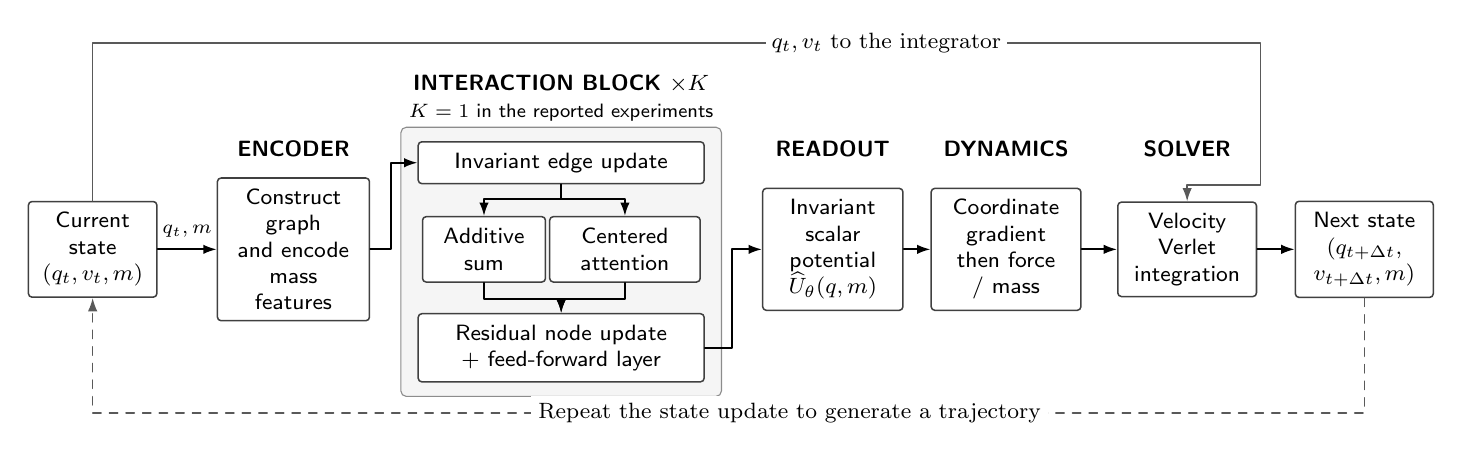
\begin{tikzpicture}[
  x=1cm,y=1cm,
  font=\sffamily\fontsize{8.2}{9.5}\selectfont,
  box/.style={draw=black!75,rounded corners=1.3pt,fill=white,
              line width=.55pt,align=center,inner sep=4pt,minimum height=.82cm},
  stage/.style={font=\sffamily\bfseries\fontsize{8}{9}\selectfont,align=center},
  substage/.style={font=\sffamily\fontsize{7.1}{8.1}\selectfont,align=center},
  arr/.style={-{Latex[length=1.7mm,width=1.2mm]},line width=.65pt},
  aux/.style={-{Latex[length=1.7mm,width=1.2mm]},line width=.55pt,draw=black!65},
  every path/.style={line cap=round,line join=round}
]
% Widen this first gap so the input label fits between, not over, the two boxes.
\node[box,text width=1.35cm] (state) at (.70,0) {Current state\\$(q_t,v_t,m)$};
\node[box,text width=1.65cm] (encoder) at (3.25,0)
  {Construct graph\\and encode\\mass features};
\node[stage] at (3.25,1.28) {ENCODER};

\node[box,text width=3.35cm,minimum height=.53cm] (edges) at (6.65,1.10)
  {Invariant edge update};
\node[box,text width=1.28cm,minimum height=.83cm] (sum) at (5.67,0)
  {Additive\\sum};
\node[box,text width=1.63cm,minimum height=.83cm] (attn) at (7.46,0)
  {Centered\\attention};
\node[box,text width=3.35cm,minimum height=.58cm] (merge) at (6.65,-1.25)
  {Residual node update\\+ feed-forward layer};
\begin{scope}[on background layer]
  \node[draw=black!45,rounded corners=2pt,fill=black!4,
        fit=(edges)(sum)(attn)(merge),inner xsep=6pt,inner ysep=5pt] (processor) {};
\end{scope}
\node[stage] at (6.65,2.10) {INTERACTION BLOCK $\times K$};
\node[substage] at (6.65,1.73) {$K=1$ in the reported experiments};

\node[box,text width=1.50cm] (potential) at (10.10,0)
  {Invariant scalar\\potential\\$\widehat U_\theta(q,m)$};
\node[stage] at (10.10,1.28) {READOUT};
\node[box,text width=1.62cm] (force) at (12.30,0)
  {Coordinate gradient\\then force / mass};
\node[stage] at (12.30,1.28) {DYNAMICS};
\node[box,text width=1.48cm] (solver) at (14.60,0)
  {Velocity Verlet\\integration};
\node[stage] at (14.60,1.28) {SOLVER};
\node[box,text width=1.47cm] (next) at (16.85,0)
  {Next state\\$(q_{t+\Delta t},$\\$v_{t+\Delta t},m)$};

\draw[arr] (state.east) -- node[midway,above=3pt,inner sep=1pt,
  font=\fontsize{7.3}{8.2}\selectfont] {$q_t,m$} (encoder.west);
\draw[arr] (encoder.east) -- (4.49,0) |- (edges.west);
\draw[arr] (edges.south) -- (6.65,.635) -| (sum.north);
\draw[arr] (6.65,.635) -| (attn.north);
\draw[arr] (sum.south) -- (5.67,-.63) -| (merge.north);
\draw[arr] (attn.south) -- (7.46,-.63) -| (merge.north);
\draw[arr] (merge.east) -- (8.82,-1.25) |- (potential.west);
\draw[arr] (potential.east) -- (force.west);
\draw[arr] (force.east) -- (solver.west);
\draw[arr] (solver.east) -- (next.west);

% Velocities enter the solver, not the potential network.
\draw[aux] (state.north) -- (.70,2.62) -- (15.53,2.62) -- (15.53,.82)
  -- (14.60,.82) -- (solver.north);
\node[fill=white,inner sep=2pt,font=\fontsize{8}{9}\selectfont] at (10.78,2.62)
  {$q_t,v_t$ to the integrator};

% Rollout feedback is separate from stacking K interaction blocks.
\draw[aux,dashed] (next.south) -- (16.85,-2.08) -- (.70,-2.08) -- (state.south);
\node[fill=white,inner sep=2.5pt,font=\fontsize{8}{9}\selectfont] at (9.55,-2.08)
  {Repeat the state update to generate a trajectory};
\end{tikzpicture}

\end{document}
